\section{Emperical evaluation}\label{sec:experiments}

We empirically evaluate the Orphrus model and the proposed disentangled relational attention operation on a range of tasks covering different domains and modalities. For each experiment, we fix the total number of heads, and compare different configurations of Orphrus against a standard Transformer where all heads are self-attention heads. The difference in performance can be interpreted as indicating the effect of having two types of attention heads disentangling sensory and relational inforrmation. Experimental details are deferred to~\Cref{sec:appendix_experimental_details}.

\subsection{Sample Efficient Relational Reasoning: Relational Games}\label{ssec:relgames}

We begin our empirical evaluation with a benchmark contributed by~\citet{shanahanExplicitlyRelationalNeurala} for evaluating the relational reasoning capabilities of machine learning models. The dataset, called ``relational games'', consists of a family of binary classification tasks, each testing a models ability to identify a particular visual relationship among a series of objects. The input is an RGB image depicting a grid of objects, and the target is a binary classification indicating whether the particular relation holds for this input.

\aanote{add more details on tasks in appendix? add figure depicting tasks.}

We use this suite of benchmarks to evaluate the \textit{sample efficiency} of our model compared to a standard Transformer. We find that our model is significantly more sample-efficient, particularly at more difficult tasks. %This shows that the Orphrus is a strong model for discriminative relational tasks, comparing favorably to previously proposed models in this domain.

Since the input is an image, we use a ``Vision Transformer''-type architecture~\citep{dosovitskiyImageWorth16x162020} where the input image is split up into patches, flattened, then fed into the model as a sequence. We fix the total number of attention heads to 2. We compare a Vision Transformer with $n_h^{sa} = 2$ to two configurations of Orphrus: one with $n_h^{sa} = 1, n_h^{ra} = 1$ and one with $n_h^{sa} = 0, n_h^{ra} = 2$.

We evaluate learning curves by varying the size of the training set, training each model until convergence, and evaluating on a hold-out validation set. We repeat this 5 times with different random seeds to compute approximate confidence intervals. This is depicted in~\Cref{fig:relgames_learning_curves}. We find that both configurations of Orphrus are consistently more sample-efficent compared to the standard Transformer. The effect is particularly dramatic on the \texttt{match pattern} task which is the most difficult and requires identifying a ``second-order'' relation (a relation between relations).

\begin{figure}
    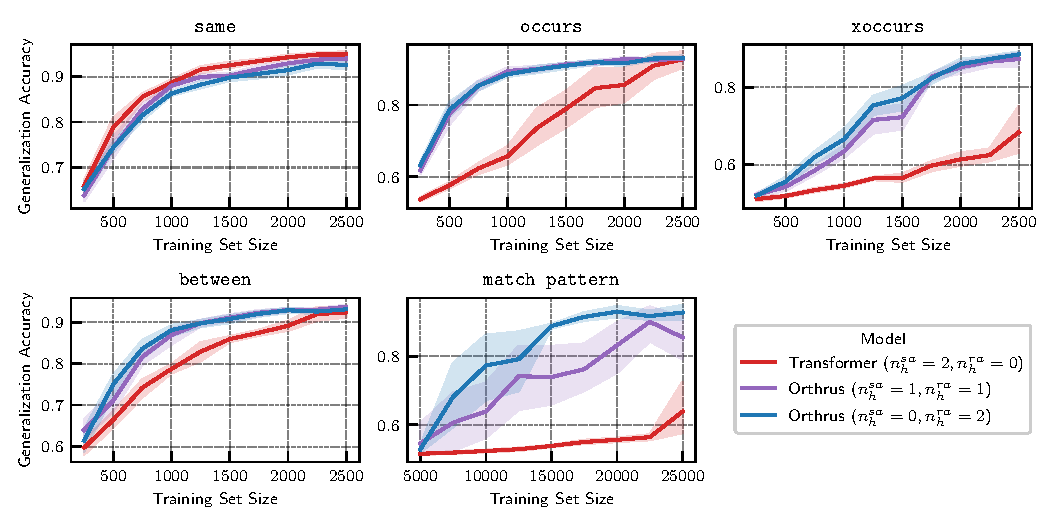
\includegraphics[width=\textwidth]{figs/experiments/relgames/relgames_learning_curves.pdf}
    \caption{Learning curves on the ``relational games'' benchmark. Orphrus is more sample-efficient compared to a Transformer with the same total number of heads. Solid lines indicate the mean over 10 trials with different random seeds and the shaded regions indicate bootstrap 95\% confidence intervals.}\label{fig:relgames_learning_curves}
\end{figure}

In this experiment, we use positional symbols as the symbol assignment mechanism since the objects can be identified through their position on the grid. We also impose symmetry on the relations in relational attention, which we find to be a useful inductive bias. Intuitively, this is because the task-relevant relations are symmetric similarity relations across different visual attributes. We provide furhter discussion and present ablations in~\Cref{sec:appendix_experimental_details}.

\aanote[margin,noinline]{legend font size is small, but medium in other figure. make consistent}

\subsection{Improved ``Symbolic Reasoning'' in Sequence-to-Sequence tasks: Mathematical Problem Solving}\label{ssec:math}

Next, we evaluate Orphrus on a set of mathematical problem-solving tasks based on the benchmark contributed by~\citet{saxtonAnalyzingMathematicalReasoning2019}. We use this as a proxy for ``symbolic reasoning''. The benchmark coonsists of a suite of mathematical problem solving datasets, with each dataset consisting of a set of question-answer pairs. The tasks range across several ``modules'' or topics including solving equations, adding polynomials, expanding polynomials, differentiating functions, predicting the next term in a sequence, etc. For example, a question might be ``\texttt{Expand (5*x - 3) * (2*x + 1).}'' with the target ``\texttt{10 * x ** 2 - x - 3}''.

This is modeled as a sequence-to-sequence model with character-level encoding. We compare Orphrus against a Transformer using matching encoder-decoder architectures. We use 2-Layer models with the total number of heads fixed to $8$ in both the encoder and the decoder. We comapre an encoder-decoder Transformer with $n_h^{sa} = 8$ against two configurations of Orphrus: one with $n_h^{sa} = 4, n_h^{ra} = 4$ for the encoder and $n_h^{sa} = 8, n_h^{ra} = 0$ for the deocder (config 1) and another with with $n_h^{sa} = 4, n_h^{ra} = 4$ for the encoder and $n_h^{sa} = 4, n_h^{ra} = 4$ for the decoder (config 2). The number of cross-attention heads is $8$ in all cases. The Orphrus models use position-relative symbols as their symbol assignment mechanism.

\begin{figure}
    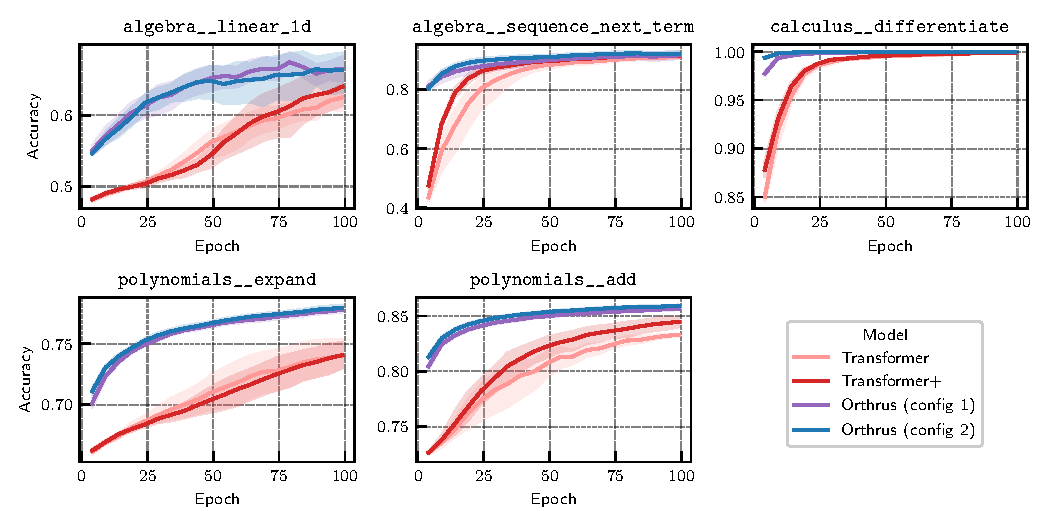
\includegraphics[width=\textwidth]{figs/experiments/math/math_training_curves_interpolation.pdf}
    \caption{Validation accuracy over the course of training on mathematical problem-solving tasks. Orphrus learns faster and reaches higher accuracy. Solid lines indicate mean over 5 trials with different random seeds, and shaded regions indicate 95\% bootstrap confidence intervals.}\label{fig:math_training_curves_interpolation}
\end{figure}

Each model is trained for 100 epochs, and accuracy on a hold-out validation set is tracked over the course of training. For each model and task, we run 5 trials with different random seeds to compute approximate confidence intervals. We find that Orphrus models learn faster and reach higher accuracies compared to a standard Transformer.

\aanote{is Transformer+ discracting? should it be removed or moved to the appendix? it does not make a noticeable difference and reviewers may ask why we don't also do this for the other experiments.}

\subsection{Language Modeling}\label{ssec:tiny_stories}

In this section, we evaluate Orphrus on autoregressive language modeling. Transformer language models are typically built on what is sometimes called a ``decoder-only'' architecture. The model receives a sequence of tokens as input and is trained to causally predict the next token at each position.

We evaluate the language modeling capabilities of Orphrus, as compared to standard Transformers, using the ``Tiny Stories'' dataset of~\citet{eldanTinyStoriesHowSmall2023}. Again, for each configuration, we fix the total number of attention heads, and compare a Transformer with only standard self-attention heads to Orphrus models with a mix of self-attention and relational attention heads. We compare a Transformer with $n_h^{sa} = 8$ attention heads to two configurations Orphrus, one with $n_h^{sa} = 6, n_h^{ra} = 2$ and another with $n_h^{sa} = 4, n_h^{ra} = 4$.

\aanote{describe context size, positional encoding, model dimension, batch size, learning rate, etc?}

\begin{figure}[ht]
    % fix d_model and vary n_layers...
    \begin{subfigure}{0.33\textwidth}
        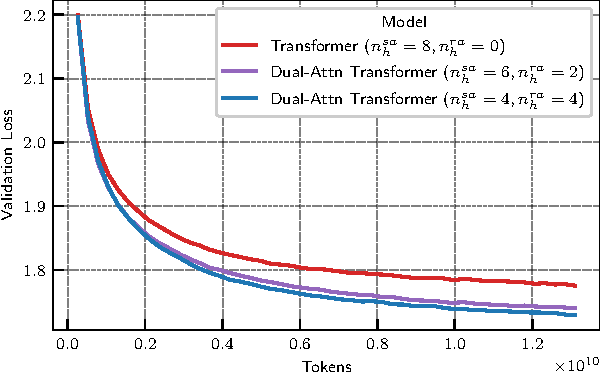
\includegraphics[width=\textwidth]{figs/experiments/tiny_stories/d64L4_symattn_asymra.pdf}
        \caption{4 Layers}
    \end{subfigure}
    \begin{subfigure}{0.33\textwidth}
        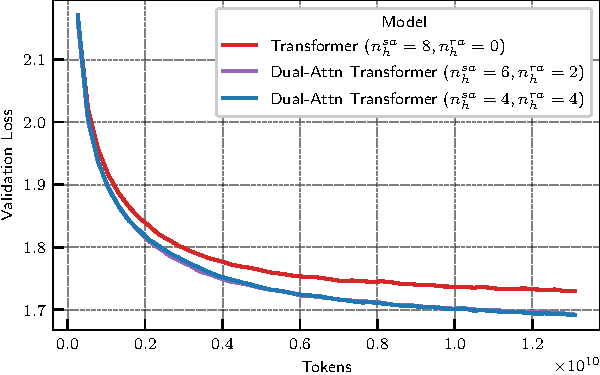
\includegraphics[width=\textwidth]{figs/experiments/tiny_stories/d64L5_symattn_asymra.pdf}
        \caption{5 Layers}
    \end{subfigure}
    \begin{subfigure}{0.33\textwidth}
        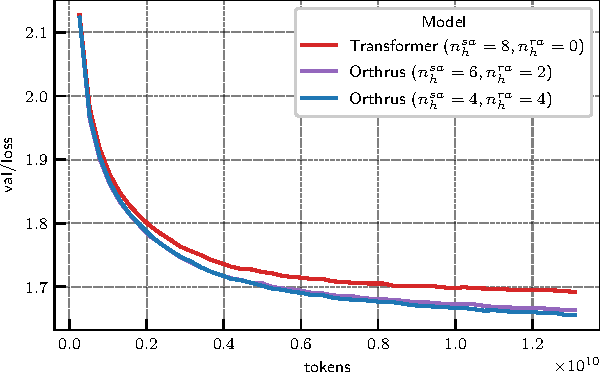
\includegraphics[width=\textwidth]{figs/experiments/tiny_stories/d64L6_symattn_asymra.pdf}
        \caption{6 Layers}
    \end{subfigure}
    \caption{Validation loss curves on a language modeling task. The $x$-axis indicates the number of tokens and the $y$-axis is the validation loss. Orphrus achieves a smaller validation loss for the same total number of attention heads.}\label{fig:tiny_stories_val_loss_curves}
\end{figure}

\Cref{fig:tiny_stories_val_loss_curves} depicts the validation loss over the course of training for each model. We find that Orphrus models with dual head attention achieve lower loss for the same total number of attention heads. The two Orphrus configurations behave similarly, with perhaps a slight advantage to $n_h^{sa} = 4, n_h^{ra} = 4$.

Here, the Orphrus models use symbolic attention as the symbol assignmnet mechanism and use asymmetric relations in relational attention. We find that symbolic attention outperforms position-relative symbols on this language modeling task. In fact, with position-relative symbols, there is no discernable advantage over the Transformer. The symbolic attention may be well-suited to language due to its implementation of a soft learnable equivalence class mapping, which can perhaps be thought of as a form of syntax. We also find the asymmetric relations in relational attention perform better than symmetric relations. We provide further discussion and present ablations in~\Cref{ssec:appendix_lm}.

We conclude this section by noting that modern large language models are applied to diverse and multi-modal tasks, where different inductive biases will be useful in different contexts. While the language models explored in this section are small, an interesting avenue for future research would be to investigate whether the observed benefits scale up to larger models. For example, one might consider a mixture-of-experts architecture~\citep{shazeer2017outrageously,fedus2022switch,duGLaM2022}, with the composition of attention head types for each expert depending on the domain.

\subsection{Multi-modality and potential in vision tasks: ImageNet}\label{ssec:imagenett}
\aanote{how is the acronym ``VAT''? Better than ViAT? VisAT? (Vision Transformer is ViT)}


here, sym\_attn performs worse than transformer, but pos-relative perhaps marginally better?